

%% This file was auto-generated by IPython.
%% Conversion from the original notebook file:
%%
\documentclass[11pt,english,a4paper]{article}
%% This is the automatic preamble used by IPython.  Note that it does *not*
%% include a documentclass declaration, that is added at runtime to the overall
%% document.
\usepackage[a4paper]{geometry}
\usepackage[cm]{fullpage}
\usepackage{amsmath}
\usepackage{amssymb}
\usepackage{graphicx}
\usepackage{ucs}
\usepackage[utf8x]{inputenc}
\usepackage{pgf}
\usepackage{tikz}
\usepackage{graphicx}

% Scale down larger images
\usepackage[export]{adjustbox}

%fancy verbatim
\usepackage{fancyvrb}
% needed for markdown enumerations to work
\usepackage{enumerate}

% Slightly bigger margins than the latex defaults
%\geometry{verbose,tmargin=3cm,bmargin=3cm,lmargin=2.5cm,rmargin=2.5cm}
\geometry{verbose,tmargin=3cm,bmargin=2cm,lmargin=1.5cm,rmargin=1.5cm}

% Define a few colors for use in code, links and cell shading
\usepackage{color}
\definecolor{orange}{cmyk}{0,0.4,0.8,0.2}
\definecolor{darkorange}{rgb}{.71,0.21,0.01}
\definecolor{darkgreen}{rgb}{.12,.54,.11}
\definecolor{myteal}{rgb}{.26, .44, .56}
\definecolor{gray}{gray}{0.45}
\definecolor{lightgray}{gray}{.95}
\definecolor{mediumgray}{gray}{.8}
\definecolor{inputbackground}{rgb}{.95, .95, .85}
\definecolor{outputbackground}{rgb}{.95, .95, .95}
\definecolor{traceback}{rgb}{1, .95, .95}

% new ansi colors
\definecolor{brown}{rgb}{0.54,0.27,0.07}
\definecolor{purple}{rgb}{0.5,0.0,0.5}
\definecolor{darkgray}{gray}{0.25}
\definecolor{lightred}{rgb}{1.0,0.39,0.28}
\definecolor{lightgreen}{rgb}{0.48,0.99,0.0}
\definecolor{lightblue}{rgb}{0.53,0.81,0.92}
\definecolor{lightpurple}{rgb}{0.87,0.63,0.87}
\definecolor{lightcyan}{rgb}{0.5,1.0,0.83}

% Framed environments for code cells (inputs, outputs, errors, ...).  The
% various uses of \unskip (or not) at the end were fine-tuned by hand, so don't
% randomly change them unless you're sure of the effect it will have.
\usepackage{framed}

% remove extraneous vertical space in boxes
\setlength\fboxsep{0pt}

% codecell is the whole input+output set of blocks that a Code cell can
% generate.

% TODO: unfortunately, it seems that using a framed codecell environment breaks
% the ability of the frames inside of it to be broken across pages.  This
% causes at least the problem of having lots of empty space at the bottom of
% pages as new frames are moved to the next page, and if a single frame is too
% long to fit on a page, will completely stop latex from compiling the
% document.  So unless we figure out a solution to this, we'll have to instead
% leave the codecell env. as empty.  I'm keeping the original codecell
% definition here (a thin vertical bar) for reference, in case we find a
% solution to the page break issue.

%% \newenvironment{codecell}{%
%%     \def\FrameCommand{\color{mediumgray} \vrule width 1pt \hspace{5pt}}%
%%    \MakeFramed{\vspace{-0.5em}}}
%%  {\unskip\endMakeFramed}

% For now, make this a no-op...
\newenvironment{codecell}{}

 \newenvironment{codeinput}{%
   \def\FrameCommand{\colorbox{inputbackground}}%
   \MakeFramed{\advance\hsize-\width \FrameRestore}}
 {\unskip\endMakeFramed}

\newenvironment{codeoutput}{%
   \def\FrameCommand{\colorbox{outputbackground}}%
   \vspace{-1.4em}
   \MakeFramed{\advance\hsize-\width \FrameRestore}}
 {\unskip\medskip\endMakeFramed}

\newenvironment{traceback}{%
   \def\FrameCommand{\colorbox{traceback}}%
   \MakeFramed{\advance\hsize-\width \FrameRestore}}
 {\endMakeFramed}

% Use and configure listings package for nicely formatted code
\usepackage{listingsutf8}
\lstset{
  language=python,
  inputencoding=utf8x,
  extendedchars=\true,
  aboveskip=\smallskipamount,
  belowskip=\smallskipamount,
  xleftmargin=2mm,
  breaklines=true,
  basicstyle=\small \ttfamily,
  showstringspaces=false,
  keywordstyle=\color{blue}\bfseries,
  commentstyle=\color{myteal},
  stringstyle=\color{darkgreen},
  identifierstyle=\color{darkorange},
  columns=fullflexible,  % tighter character kerning, like verb
}

% The hyperref package gives us a pdf with properly built
% internal navigation ('pdf bookmarks' for the table of contents,
% internal cross-reference links, web links for URLs, etc.)
\usepackage{hyperref}
\hypersetup{
  breaklinks=true,  % so long urls are correctly broken across lines
  colorlinks=true,
  urlcolor=blue,
  linkcolor=darkorange,
  citecolor=darkgreen,
  }
\usepackage{helvet}
\renewcommand{\familydefault}{\sfdefault}
% hardcode size of all verbatim environments to be a bit smaller
\makeatletter 
\g@addto@macro\@verbatim\small\topsep=0.5em\partopsep=0pt
\makeatother 

% Prevent overflowing lines due to urls and other hard-to-break entities.
\sloppy




\begin{document}


\title{Electricity Authority Weekly Report}
\author{Market Performance team}
\maketitle
\thispagestyle{empty}
\begin{tikzpicture}[remember picture,overlay]
    \node (kinmap) [xshift=0.5cm,yshift=0.5cm] at (current page.south west) [above right] {\includegraphics[width=19.75cm]{footer.png}};
\end{tikzpicture}

\begin{tikzpicture}[remember picture,overlay]
    \node (kinmap) [xshift=-0.5cm,yshift=-0.5cm] at (current page.north east) [below left] {\includegraphics[width=8cm]{ea-logo-medium.jpg}};
\end{tikzpicture}

\newpage


\section{Hydro Risk Curves and current storage situation}
\vspace{1cm}
\begin{center}
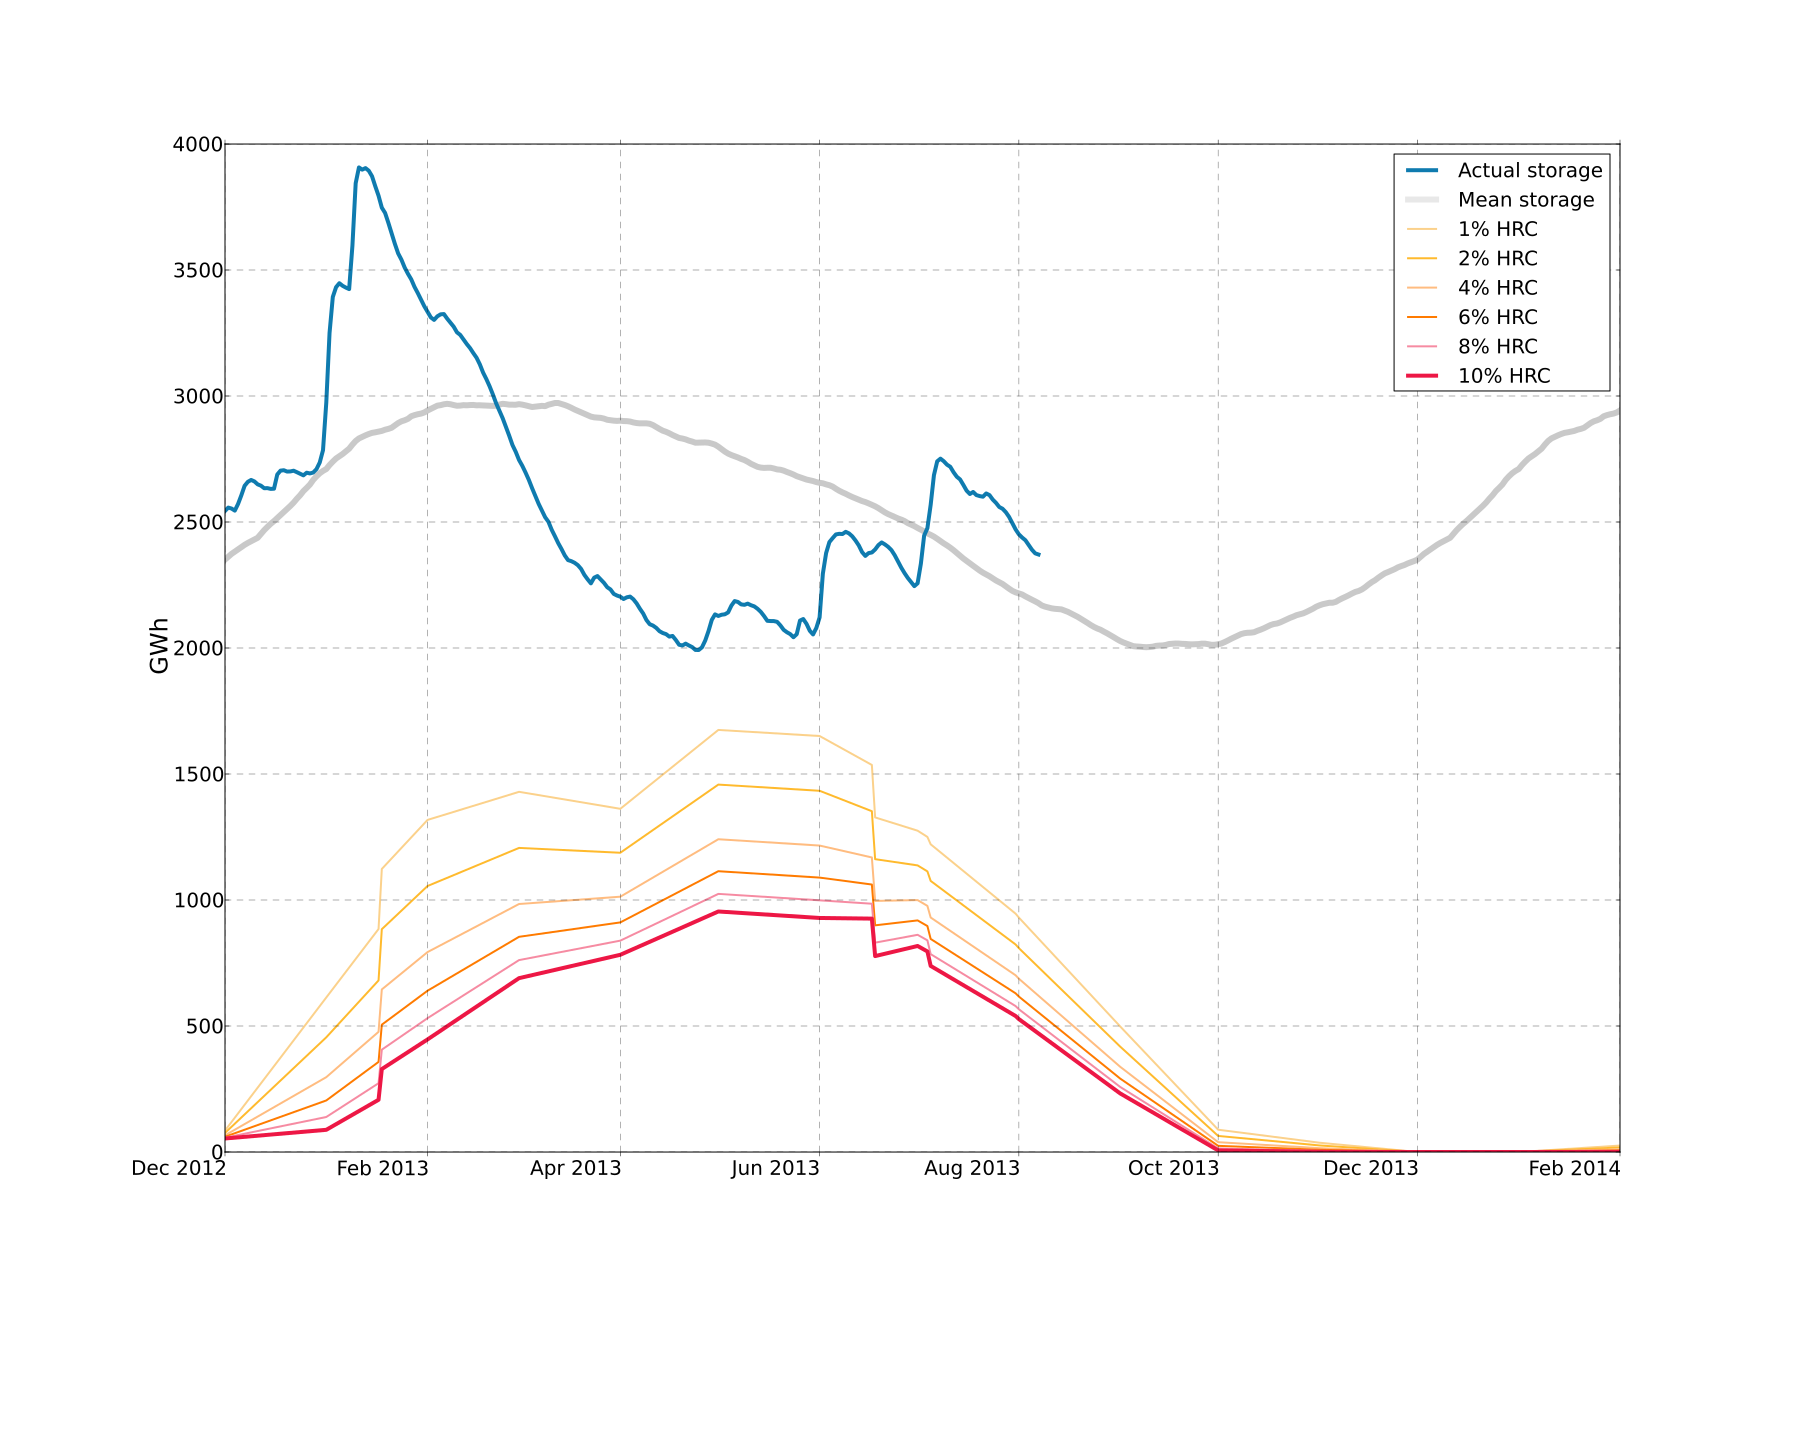
\includegraphics[max size={\textwidth}{0.9\textheight}]{figures/hrc.pdf}
\end{center}



\subsection{NZ total storage and inflows over past year}
\vspace{5mm}

\begin{center}
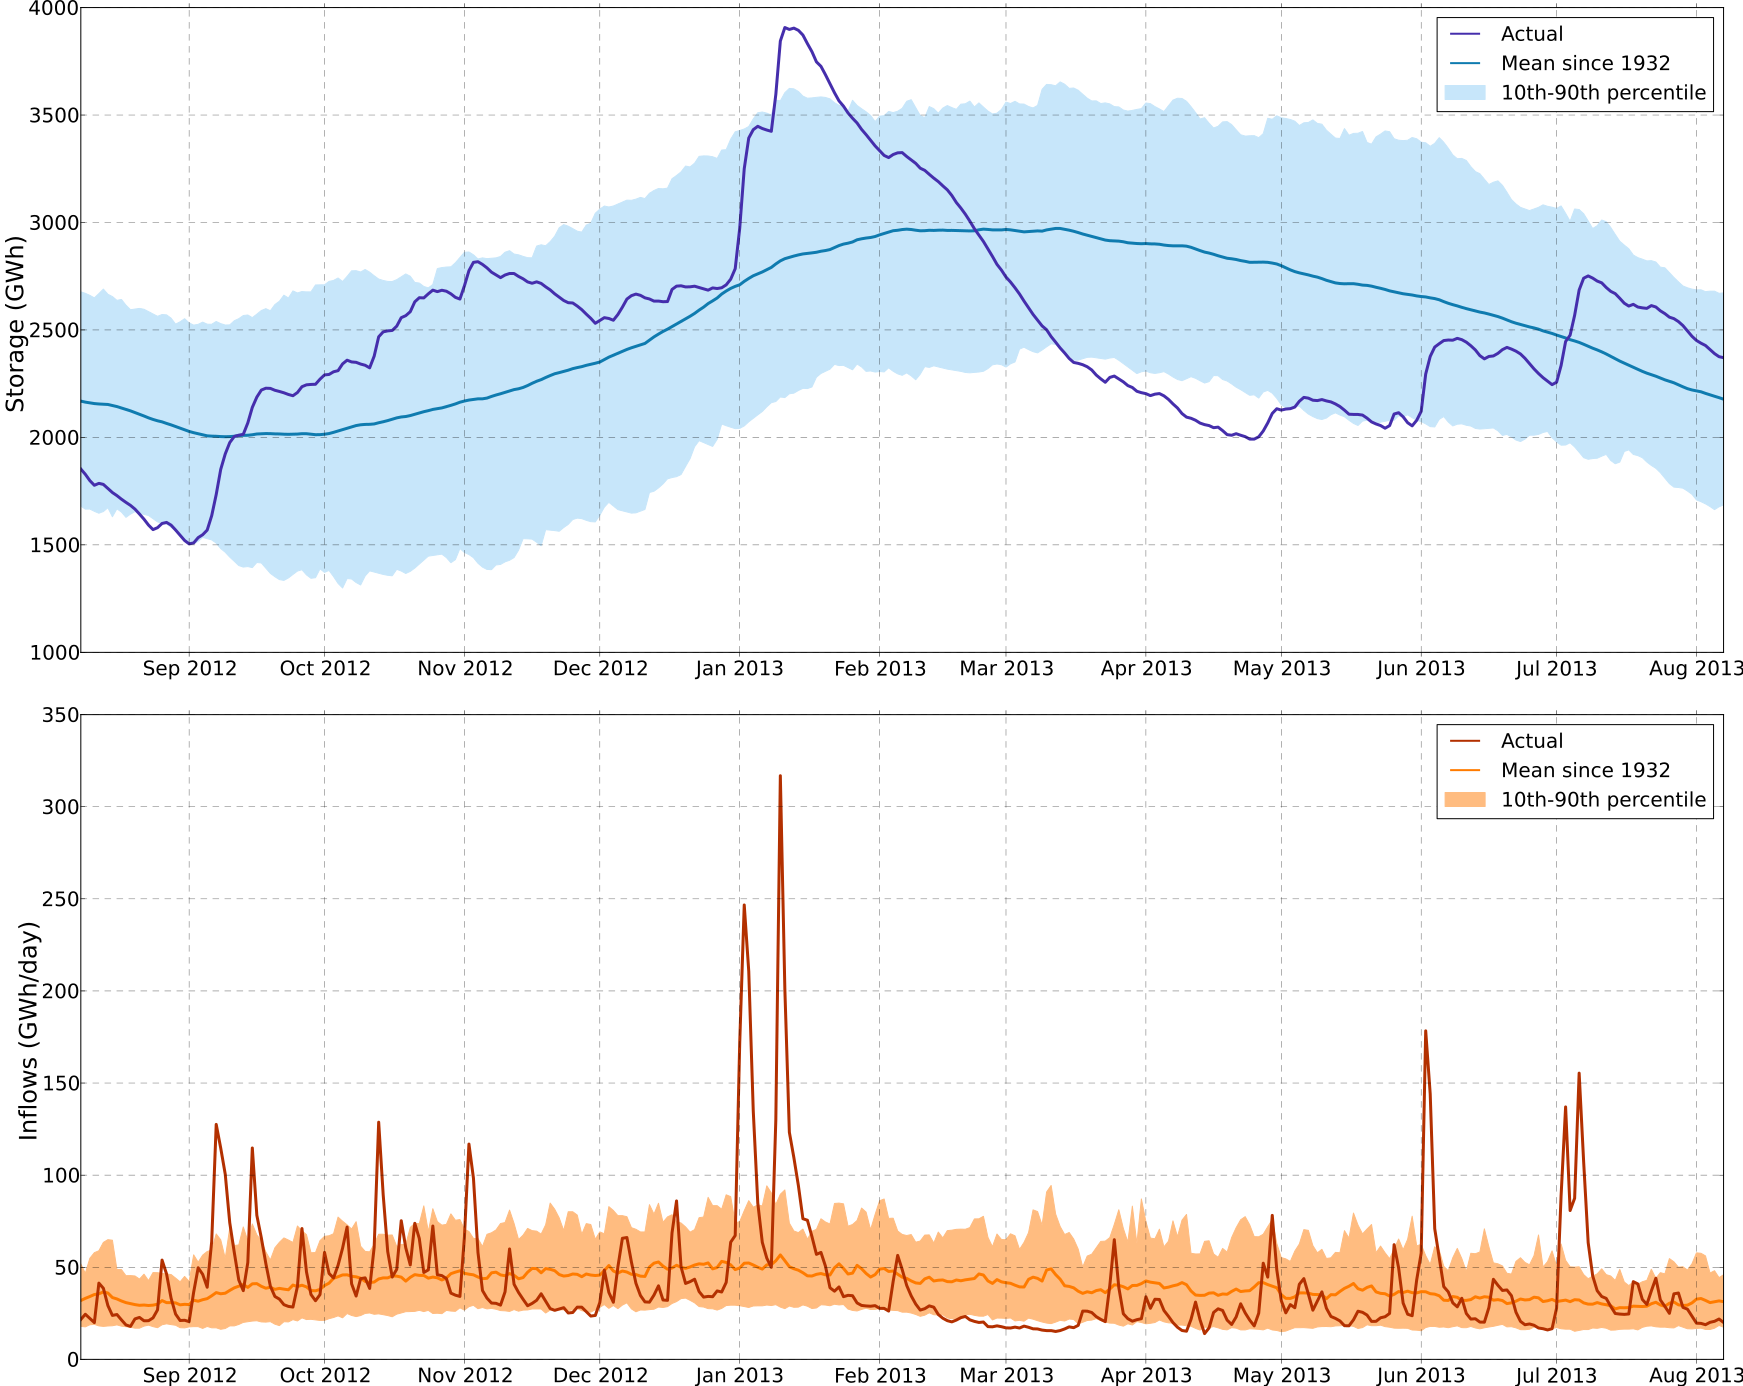
\includegraphics[max size={\textwidth}{0.9\textheight}]{figures/nz.pdf}
\end{center}

\vspace{5mm}

\subsection{Lake Taupo total storage and inflows over past year}
\begin{center}
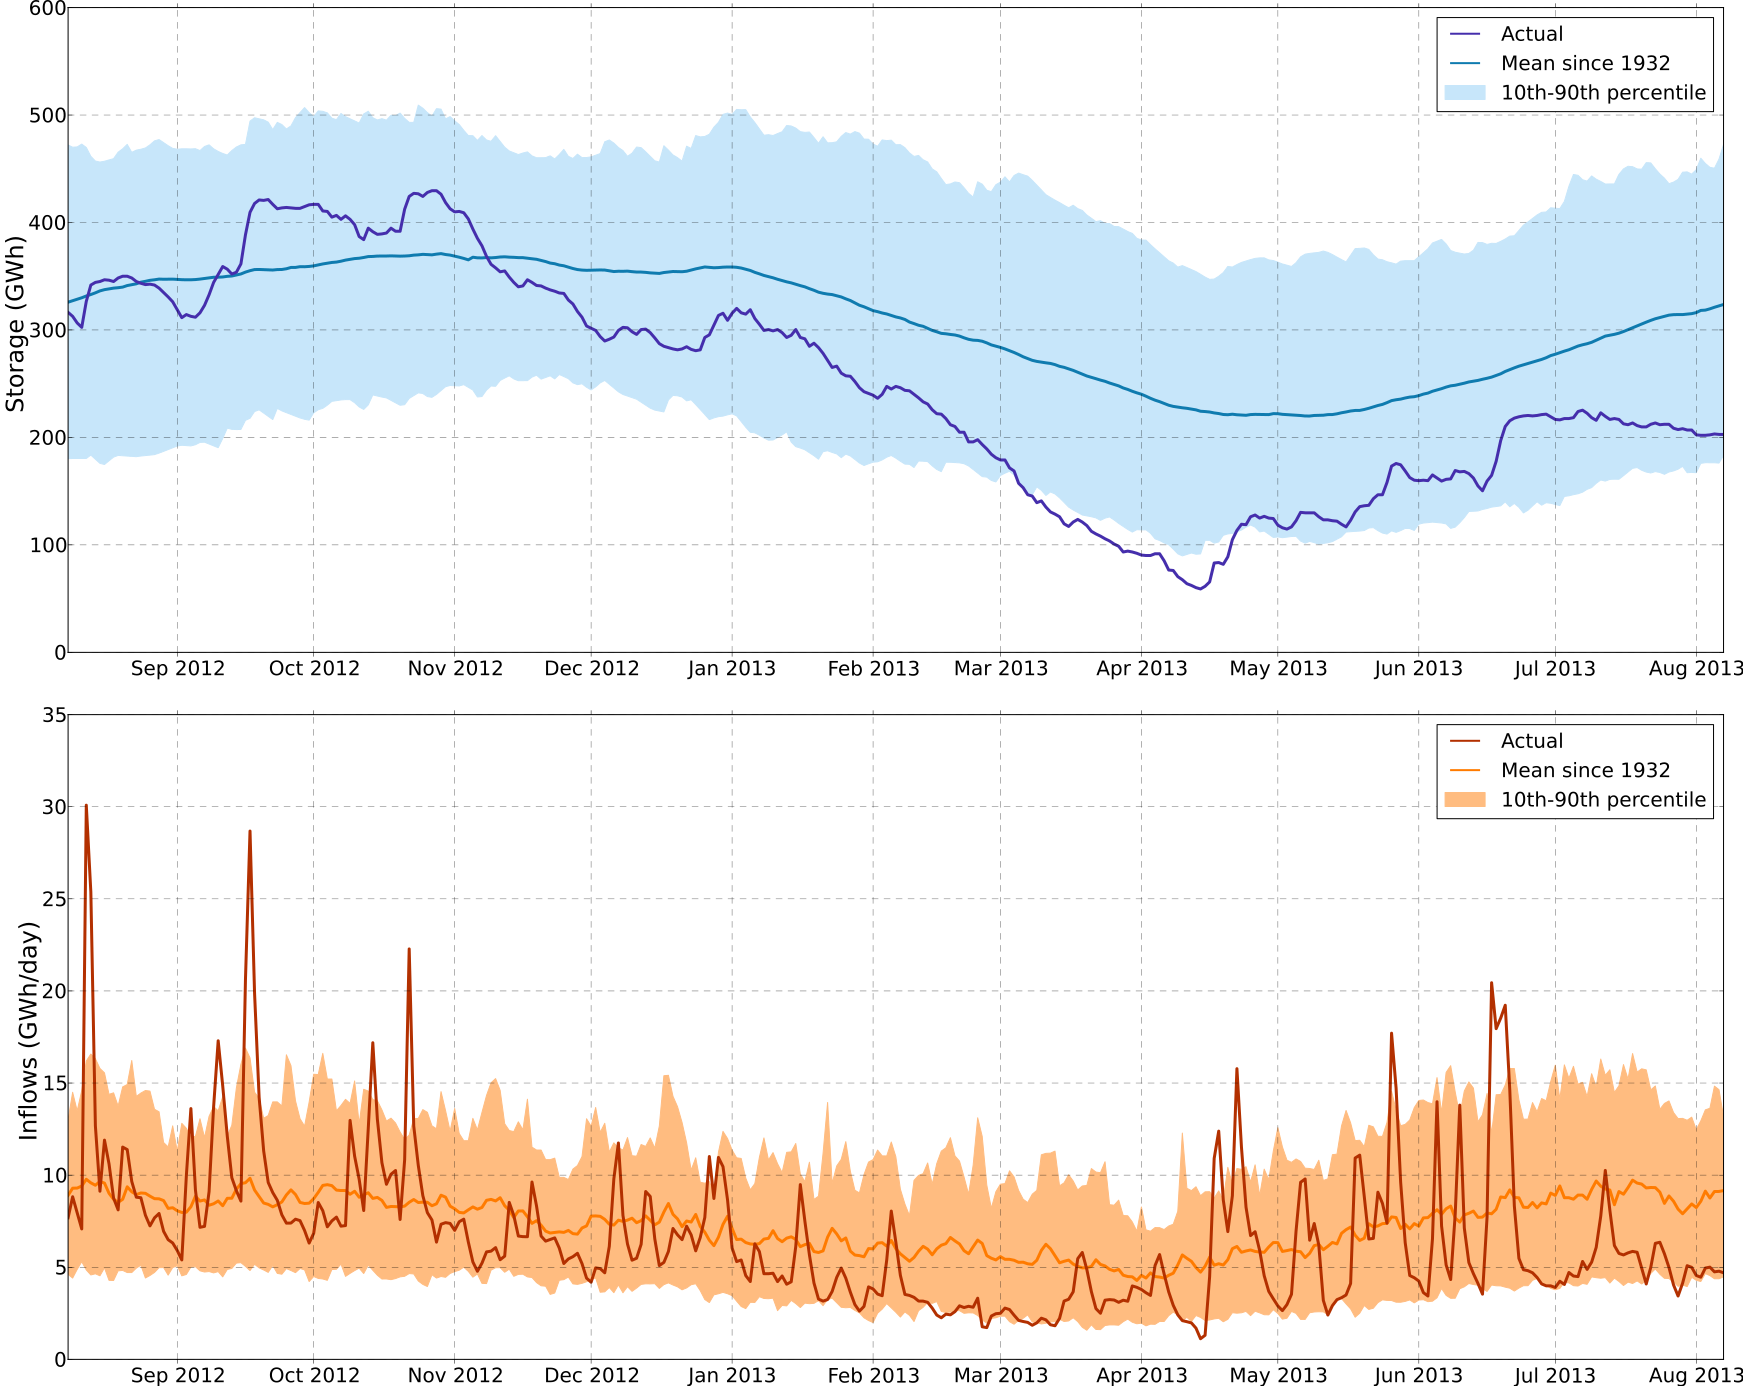
\includegraphics[max size={\textwidth}{0.9\textheight}]{figures/taupo.pdf}
\end{center}


\subsection{Lake Tekapo total storage and inflows over past year}
\begin{center}
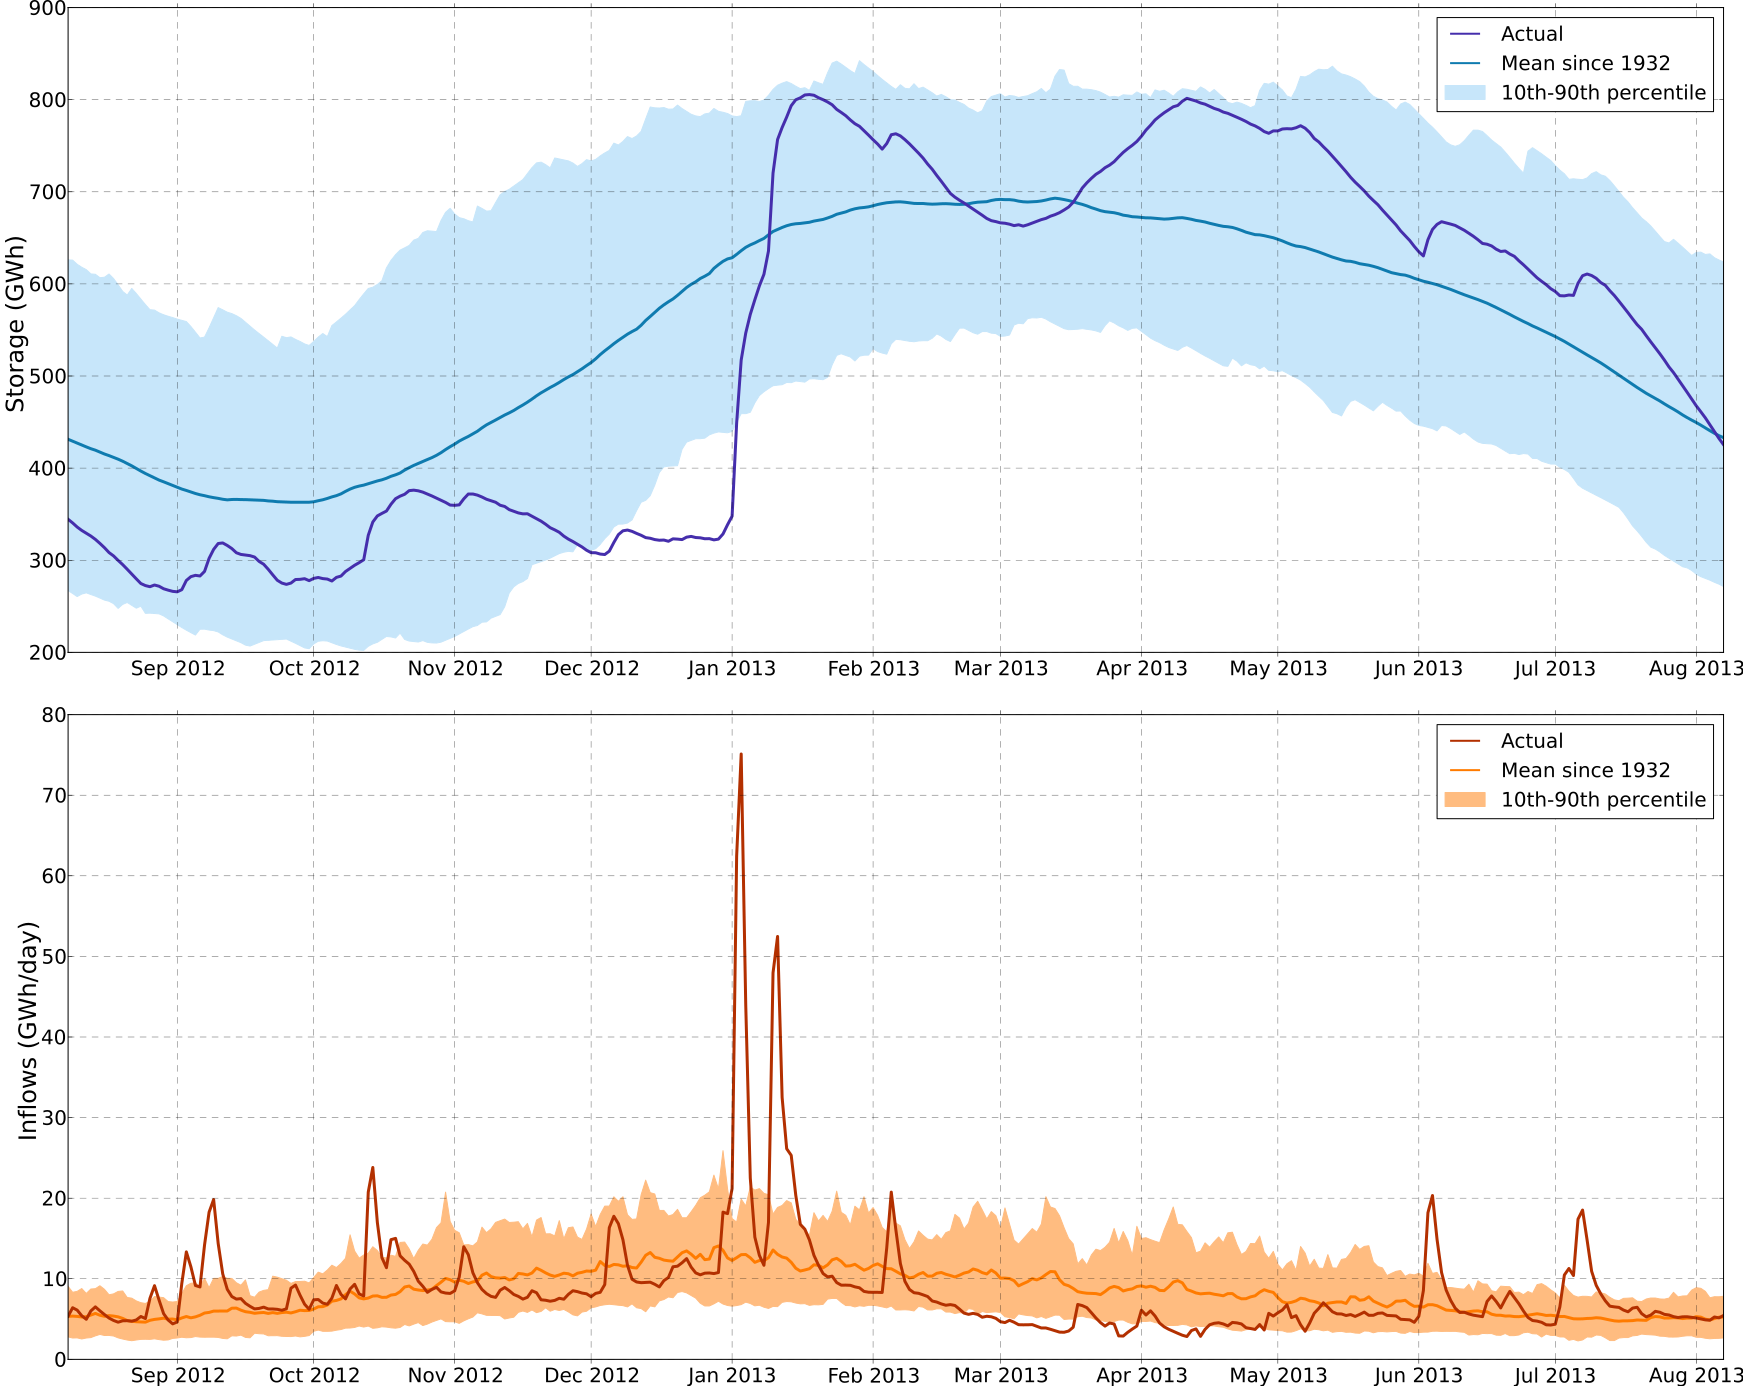
\includegraphics[max size={\textwidth}{0.9\textheight}]{figures/tekapo.pdf}
\end{center}

\vspace{5mm}

\subsection{Lake Pukaki total storage and inflows over past year}
\begin{center}
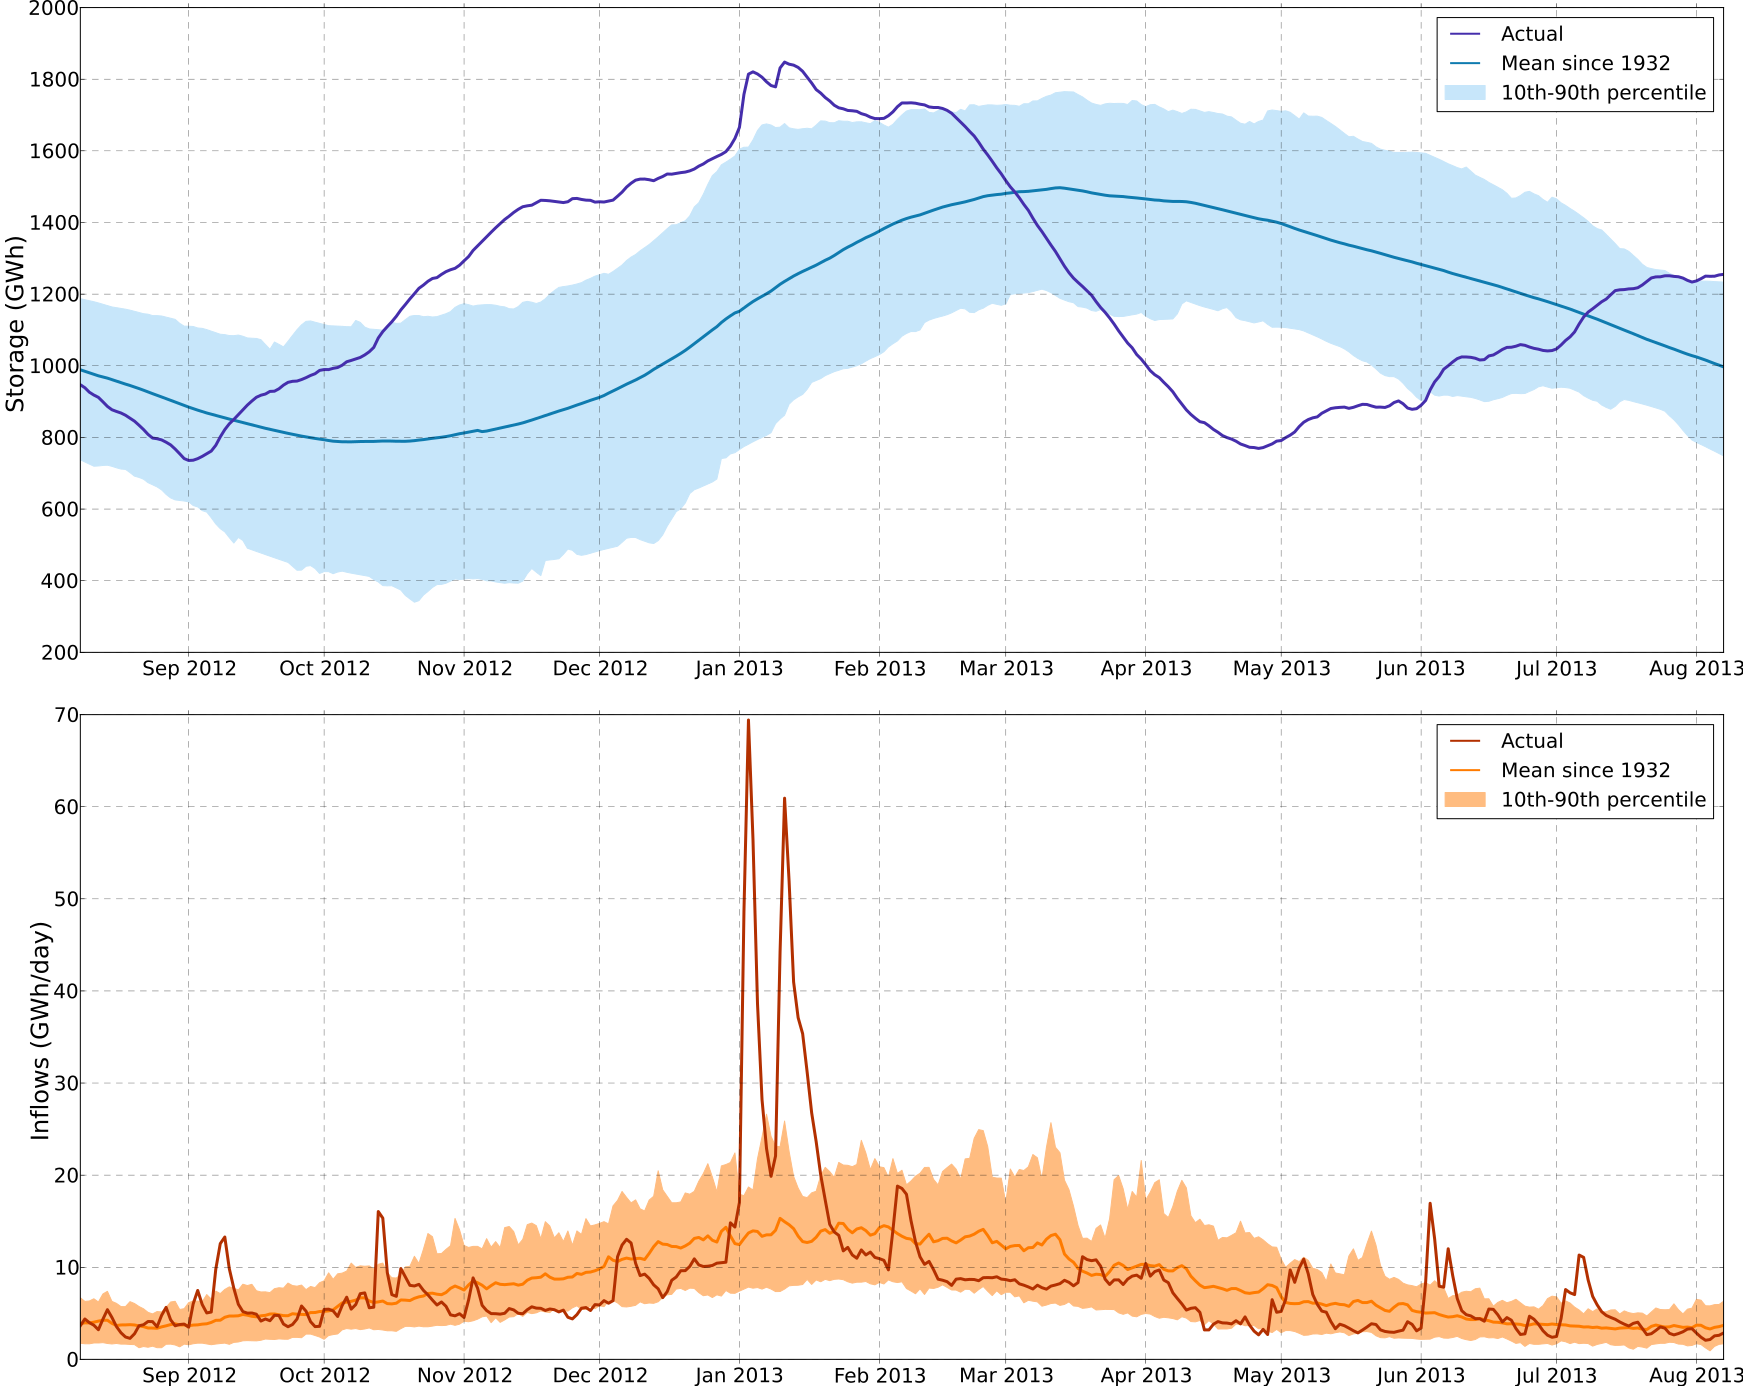
\includegraphics[max size={\textwidth}{0.9\textheight}]{figures/pukaki.pdf}
\end{center}


\subsection{Lake Hawea total storage and inflows over past year}
\vspace{5mm}

\begin{center}
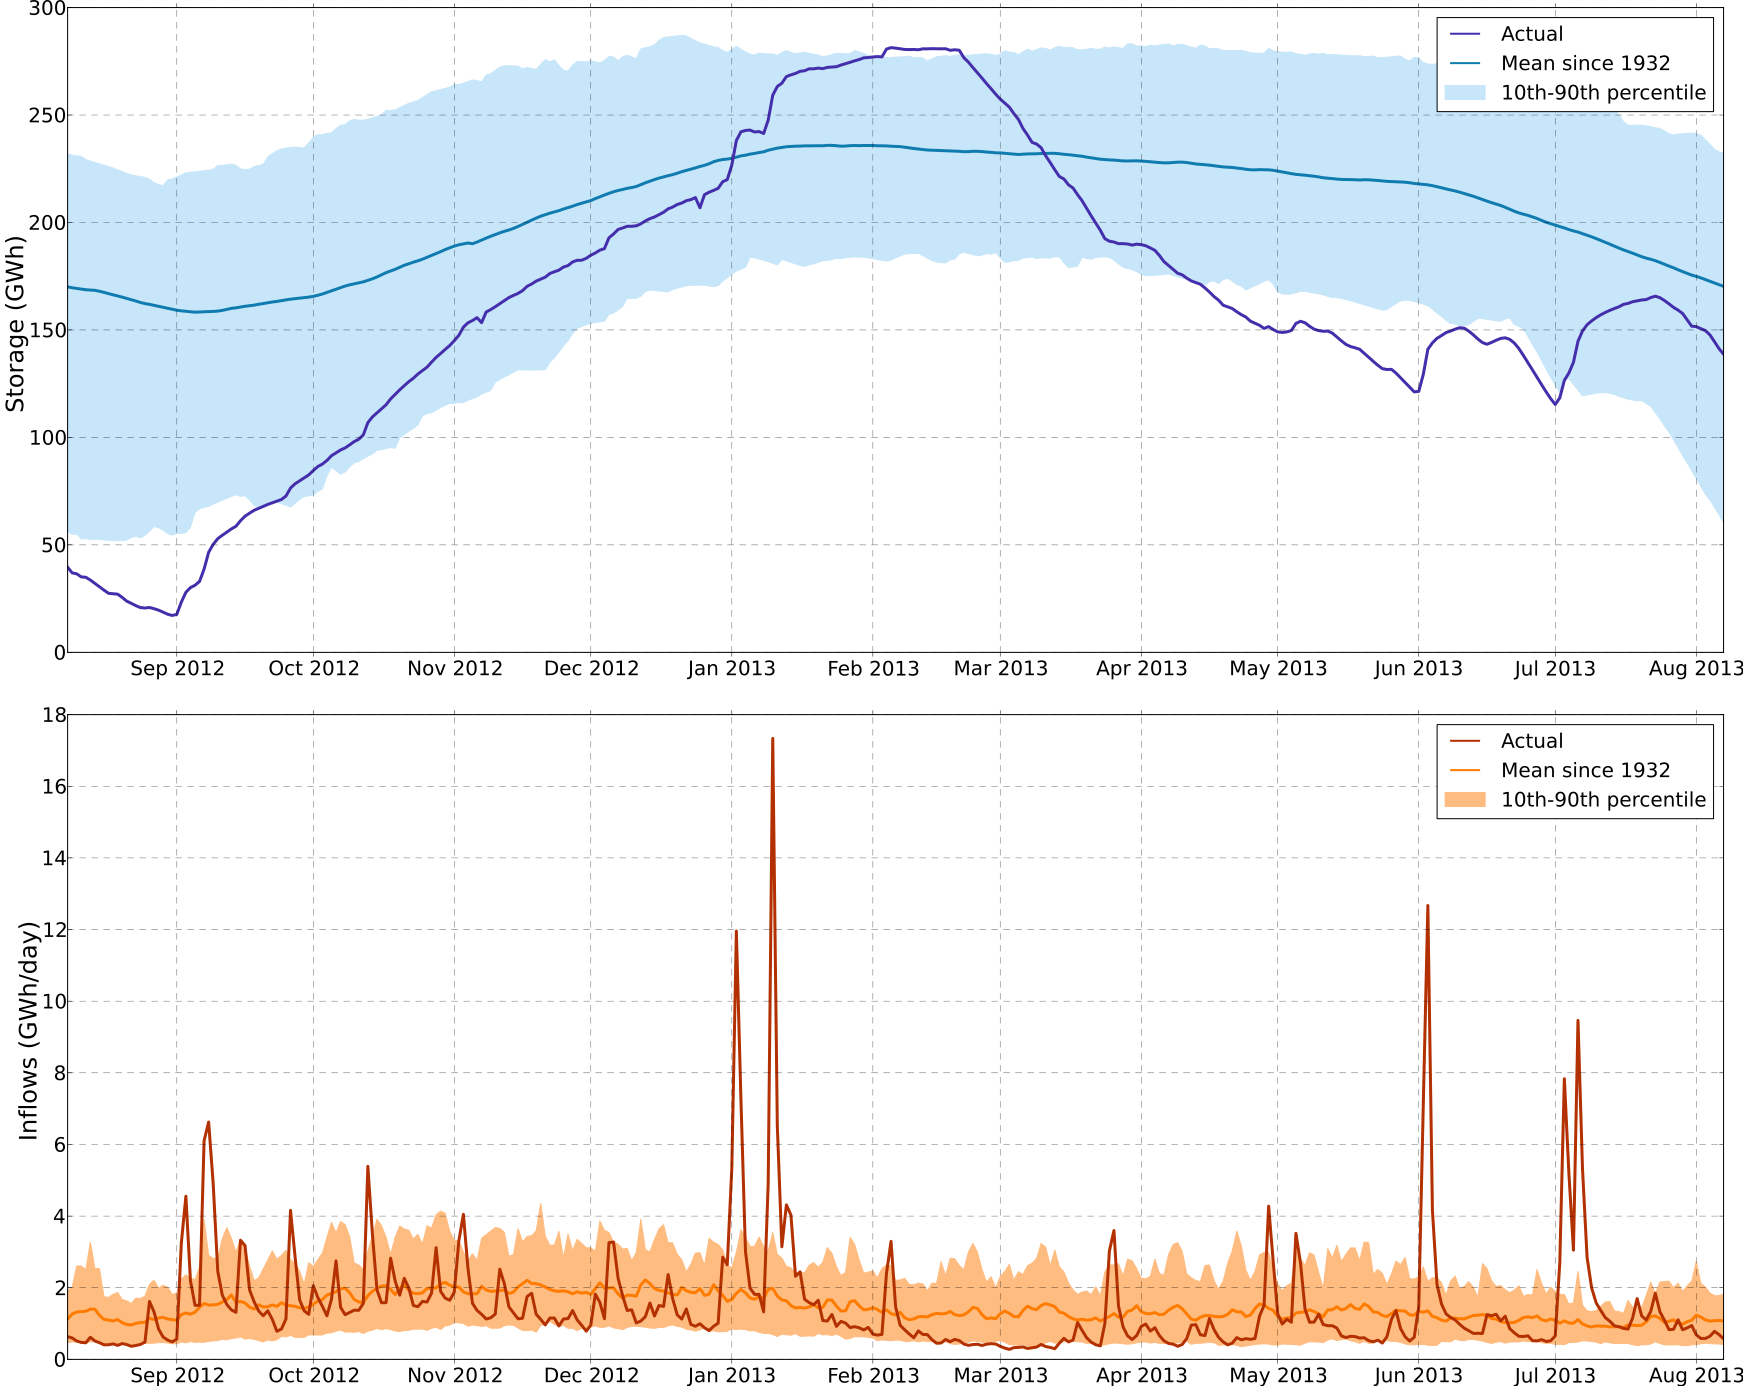
\includegraphics[max size={\textwidth}{0.9\textheight}]{figures/hawea.pdf}
\end{center}

\vspace{5mm}

\subsection{Lake Te Anau and Manapouri total storage and inflows over
past year}
\begin{center}
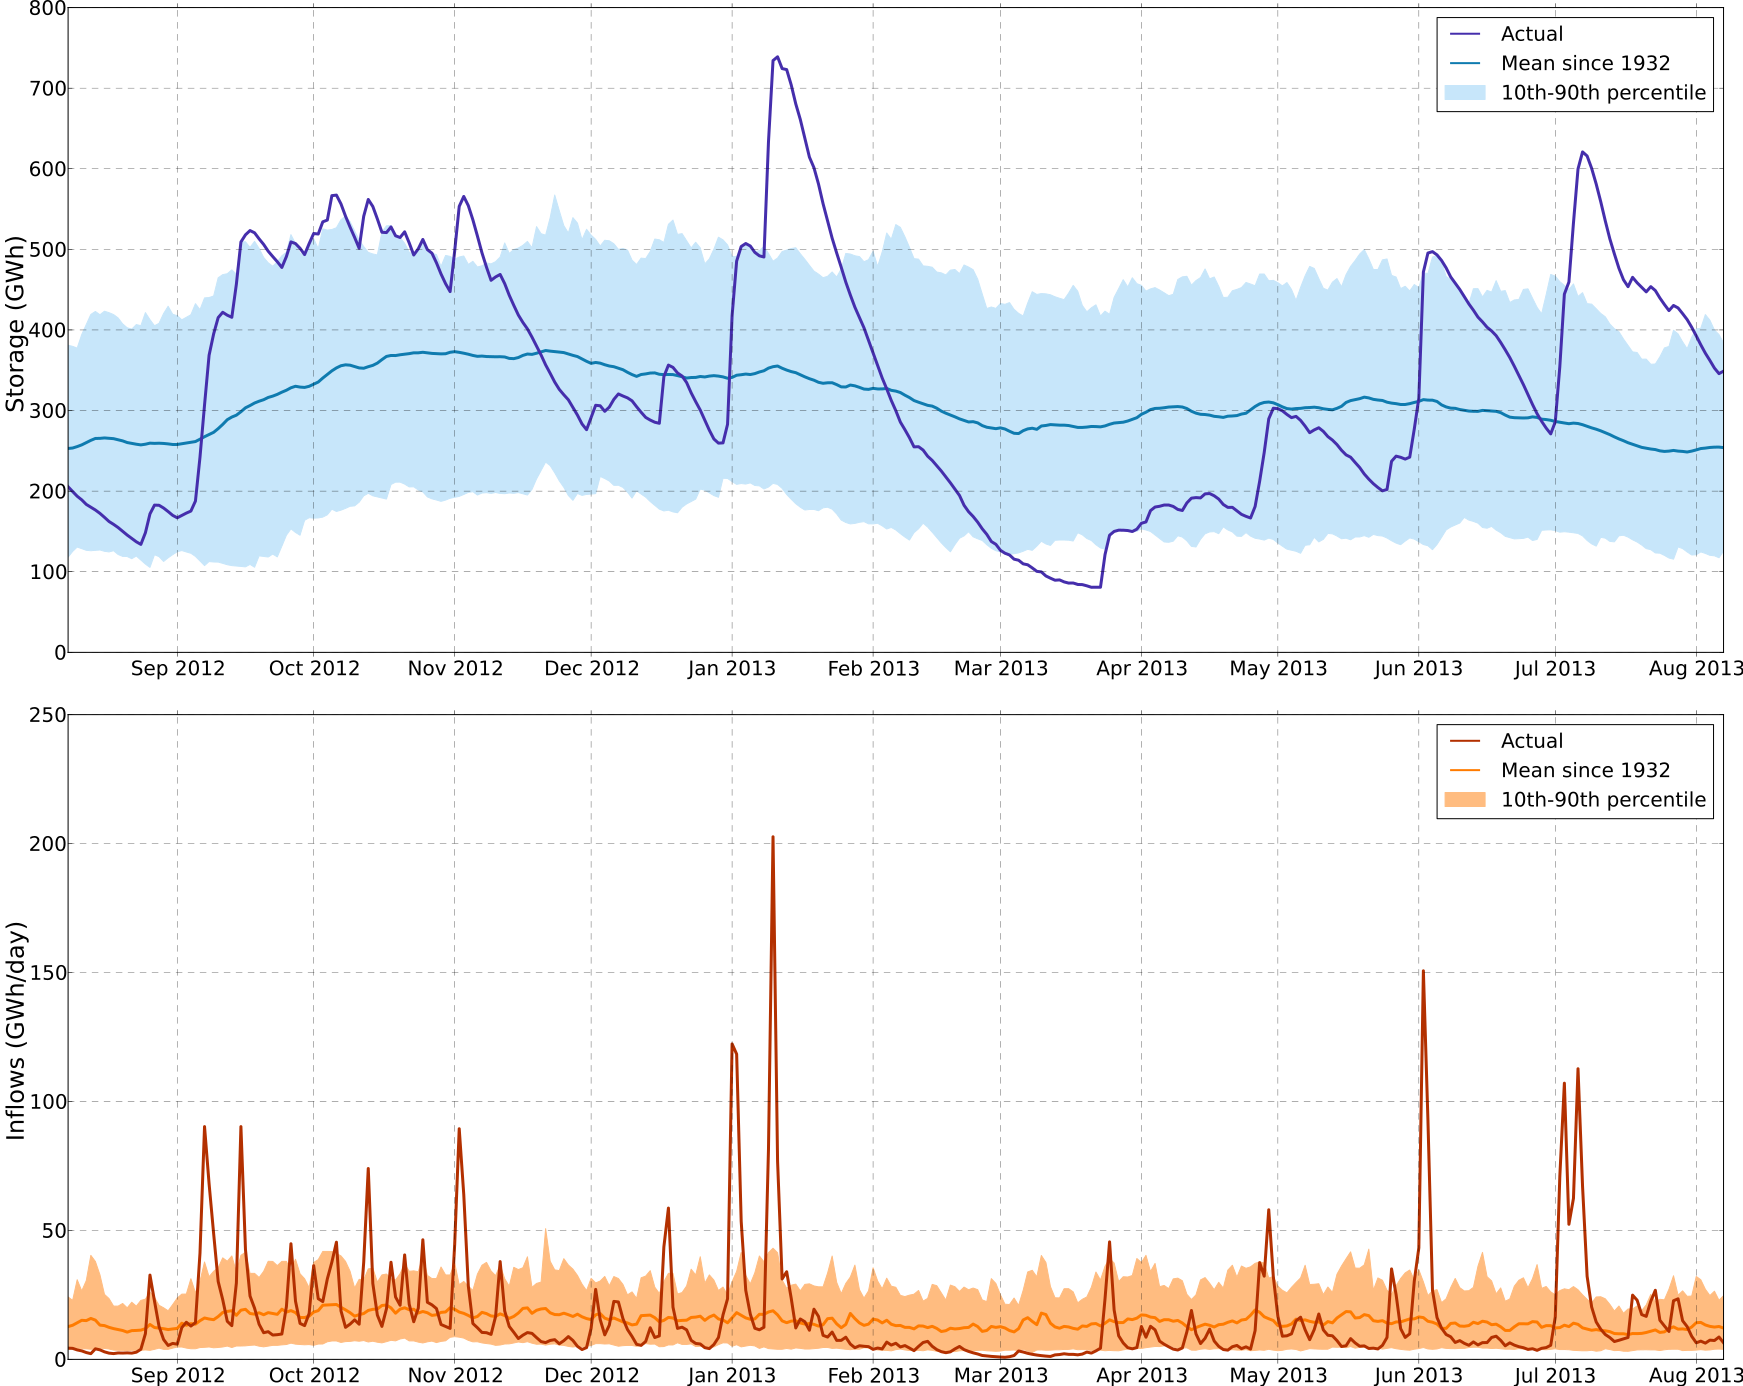
\includegraphics[max size={\textwidth}{0.9\textheight}]{figures/teanaumanapouri.pdf}
\end{center}

\subsection{Snow Storage}
\begin{center}
\includegraphics[max size={0.8\textwidth}{0.8\textheight}]{figures/snow.png}
\end{center}


\subsection{Rainfall outlook}
\begin{center}
\includegraphics[max size={\textwidth}{0.9\textheight}]{figures/niwa.png}
\end{center}


\section{Three month demand weighted price comparison}
\vspace{2cm}

\begin{center}
\includegraphics[max size={0.95\textwidth}{0.9\textheight}]{figures/lwap.pdf}
\end{center}

\newpage
\section{Hedge Market}

\subsection{Forward Price Curve -- Otahuhu}

\begin{center}
\includegraphics[max size={0.95\textwidth}{0.9\textheight}]{figures/ota_fpc.pdf}
\end{center}

\subsection{Forward Price Curve -- Benmore}

\begin{center}
\includegraphics[max size={0.95\textwidth}{0.9\textheight}]{figures/ben_fpc.pdf}
\end{center}

\subsection{Current quarter trends}

\begin{center}
\includegraphics[max size={\textwidth}{0.9\textheight}]{figures/cq_trend.pdf}
\end{center}


\subsection{Monthly Volumes}

\begin{center}
\includegraphics[max size={\textwidth}{0.9\textheight}]{figures/asx_volumes.pdf}
\end{center}

\subsection{Open Interest}
\vspace{2cm}
\begin{center}
\includegraphics[max size={\textwidth}{0.9\textheight}]{figures/asx_opint.pdf}
\end{center}

\subsection{Trends over last year - Otahuhu}

\begin{center}
\includegraphics[max size={\textwidth}{0.9\textheight}]{figures/asx_ota_year.pdf}
\end{center}

\subsection{Trends over last year - Benmore}

\begin{center}
\includegraphics[max size={\textwidth}{0.9\textheight}]{figures/asx_ben_year.pdf}
\end{center}

\subsection{Trends over last year - Benmore minus Otahuhu}

\begin{center}
\includegraphics[max size={0.825\textwidth}{0.9\textheight}]{figures/asx_ben_minus_ota_year.pdf}
\end{center}

\end{document}

